\documentclass[a4paper, 12pt]{report}

\usepackage[a4paper, total={6in, 9in}]{geometry}
\usepackage{lmodern} % Police standard sous LaTeX : Latin
\usepackage[english]{babel} % Pour la langue anglaise
\usepackage[utf8]{inputenc} % Pour l'UTF-8
\usepackage[T1]{fontenc} % Pour les césures des caractères
\usepackage{graphicx}
\usepackage{subfig}
\usepackage{ragged2e}
\justifying

\renewcommand{\thesection}{\Alph{section}}

\title{Model of the spread of a disease in a population of mobile agents}
\author{NIDDAM Benjamin}
\date{\today}

\begin{document}
\begin{titlepage}
	\maketitle
\end{titlepage}

\newpage

\tableofcontents

\newpage
\section{Introduction}
The modeling of spatial segregation proposed in the 1970s by Thomas
C. Schelling made an impression because of the perverse effect she suggested: a strong
segregation could be the collective result of individual decisions that are not aimed at
such segregation. We would be dealing with an almost spontaneous phenomenon. The problem is
that such a conclusion outright contradicts the entropy principle. An exam
more attentive to the model makes it possible here to identify no less than four biases which condition the
results. We will study here the impacts that population density and the dissatisfaction rate can have on segregation.

\section{Model presentation}

Schelling's model is a model of spatial segregation. It takes the form of a matrix of n * n boxes.
Each cell is represented by an integer between -1, 0 and 1. Empty cells are represented by 0 while cells
occupied by an individual are represented by a -1 or 1. We therefore obtain a stylized representation of two populations which
share an urban area.

Initially, the agents are placed at random to simulate the mix of populations. We then add a rule of
movement of agents: they will change boxes if, in their immediate neighborhood, there is not at least "n"
agents of the same type as them. When an agent is not satisfied, we generate a random place among the empty cells and we
place the agent in this box; which frees up its old place. This operation is carried out until all the agents
are satisfied, or until the defined maximum time is reached. Under these conditions, we obtain groupings of
populations which appeared without being intentionally provoked.

% \newpage

\begin{figure}[!h]

	\centering
	\subfloat{{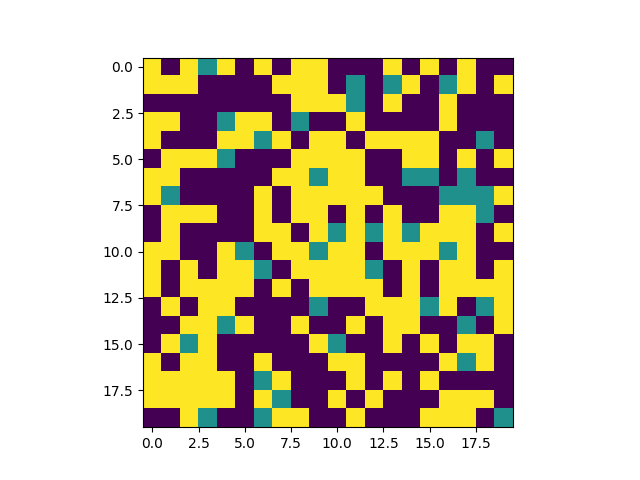
\includegraphics[width=7cm]{../resultats/worlds/Init/INS_0.6/initial_20.png} }}
	\centering
	\subfloat{{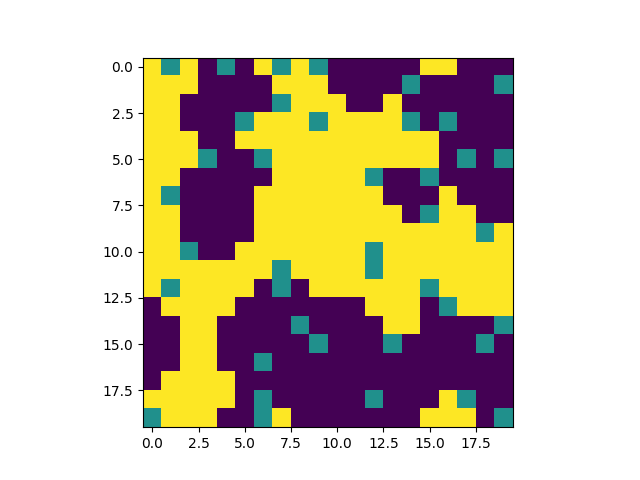
\includegraphics[width=7cm]{../resultats/worlds/Sorted/INS_0.6/sorted_20.png} }}
	\caption{Graphic representations of the initial and segregated populations with Schelling's model}

\end{figure}

\newpage

\section{Experiments, results}

With this model, we were able to study the effects of population density and the dissatisfaction rate on the movements of
the agents.

\subsection{Population density}

As said, we have run several simulations with different population density values. In other words,
we wanted to study whether the number of free sites played a role in the separation of populations.

\vspace{0.7cm}

We varied the number of free cells from 15 to 25 and obtained the following results:

\begin{figure}[!h]
	\centering
	\subfloat[Initial state]{{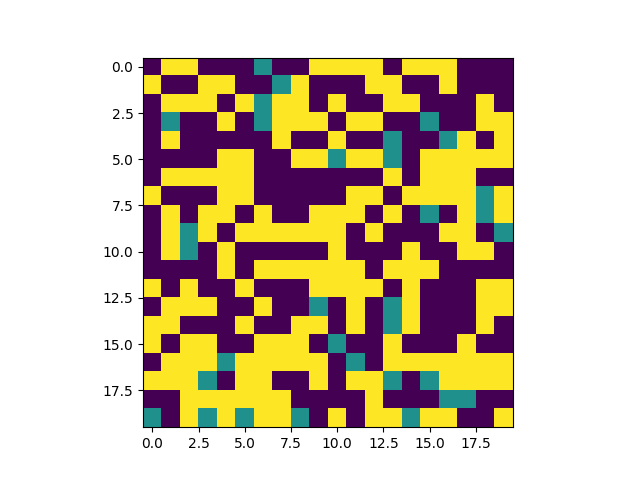
\includegraphics[width=7cm]{../resultats/worlds/Init/INS_0.5/initial_16.png} }}
	\subfloat[Population segregation after simulation]{{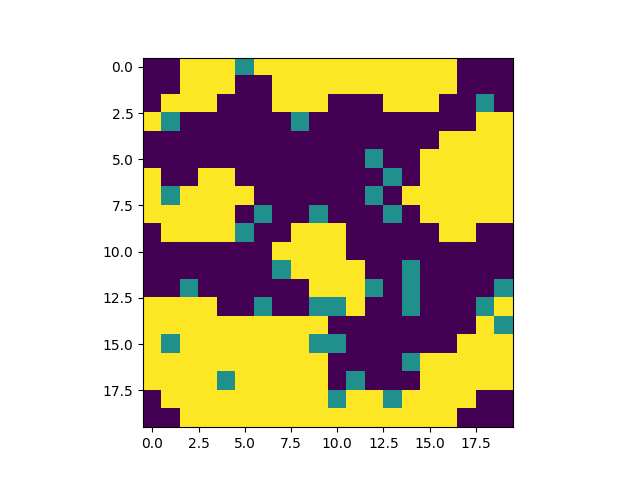
\includegraphics[width=7cm]{../resultats/worlds/Sorted/INS_0.5/sorted_16.png} }}
	\caption{Graphic representations of the initial and segregated states of Schelling's model with 16 free cells over 400 at differents dissatisfaction rates}
\end{figure}

\begin{figure}[!h]
	\centering
	\subfloat[Initial state]{{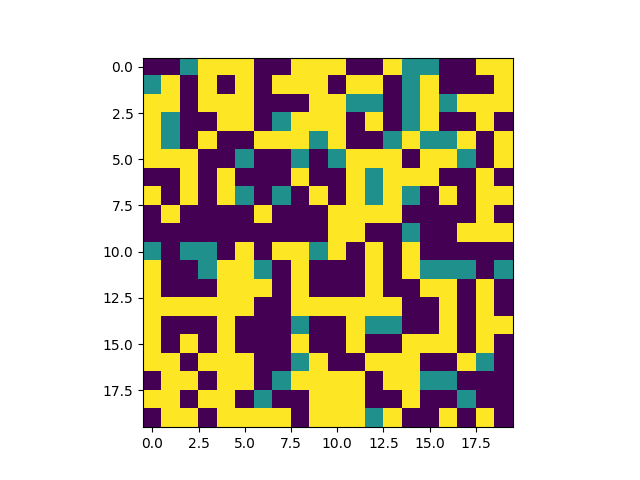
\includegraphics[width=7cm]{../resultats/worlds/Init/INS_0.5/initial_24.png} }}
	\subfloat[Population segregation after simulation]{{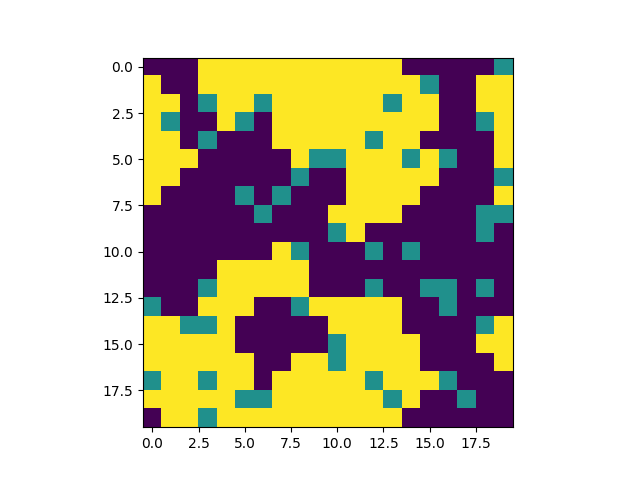
\includegraphics[width=7cm]{../resultats/worlds/Sorted/INS_0.5/sorted_24.png} }}
	\caption{Graphic representations of the initial and segregated states of Schelling's model with 24 free cells over 400 at differents dissatisfaction rates}

\end{figure}

\newpage

It is observed that in both cases, the agents separated into two distinct groups according to their color. So we have
represented the time taken by our agents to arrive at a stable situation according to the population density.

\begin{figure}[!h]
	\centering
	\subfloat[dissatisfaction rate: 0.2]{{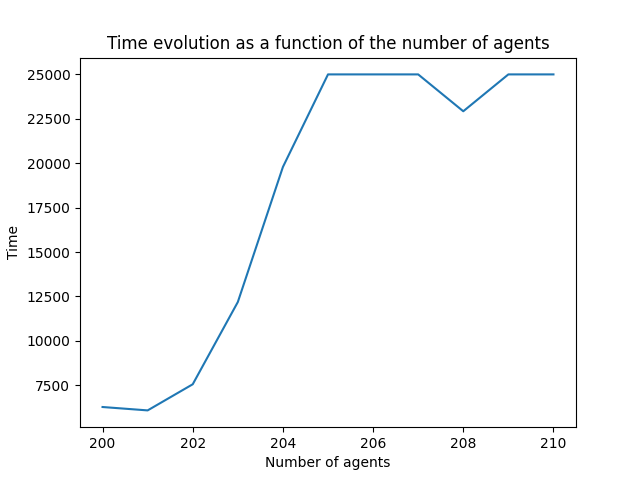
\includegraphics[width=7cm]{../resultats/Curves/POP_evolution/time_evolution_as_a_function_of_libre_INS_0.2.png} }}
	\subfloat[dissatisfaction rate: 0.3]{{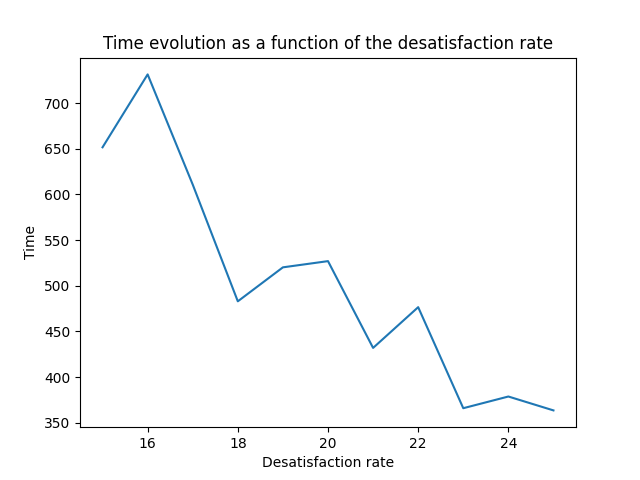
\includegraphics[width=7cm]{../resultats/Curves/POP_evolution/time_evolution_as_a_function_of_libre_INS_0.3.png} }}
\end{figure}
\begin{figure}[!h]
	\centering
	\subfloat[dissatisfaction rate: 0.4]{{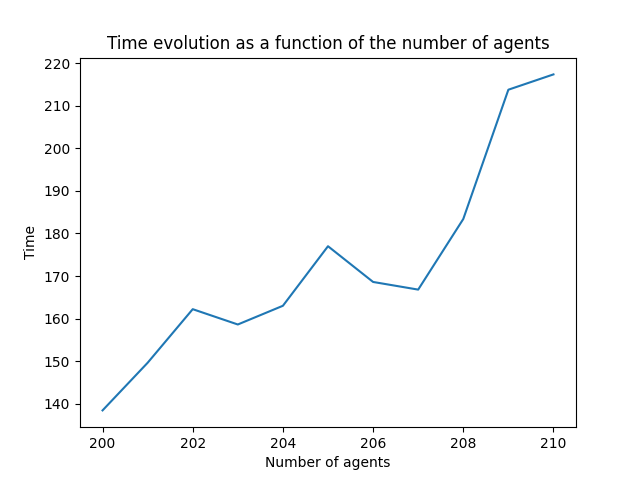
\includegraphics[width=7cm]{../resultats/Curves/POP_evolution/time_evolution_as_a_function_of_libre_INS_0.4.png} }}
	\caption{Graphic representations of the time spent by the agents to reach a stable state with a variable population density with an dissatisfaction rate of 0.3}
\end{figure}


We can see that the convergence time towards a stable state is longer as the population density increases. This is due to the decrease of the number of
free cells. We can therefore conjecture that population density plays a role in the separation of our population. Let's try something else.
\newpage

\subsection{Dissatisfaction rate}

This time we have varied the dissatisfaction rate over a range of values from 0.2 to 0.8 with a step of 0.1. For these seven simulations, we obtained
very different results from each other:

\begin{figure}[!h]
	\centering
	\subfloat[Dissatisfaction rate at 0.1]{{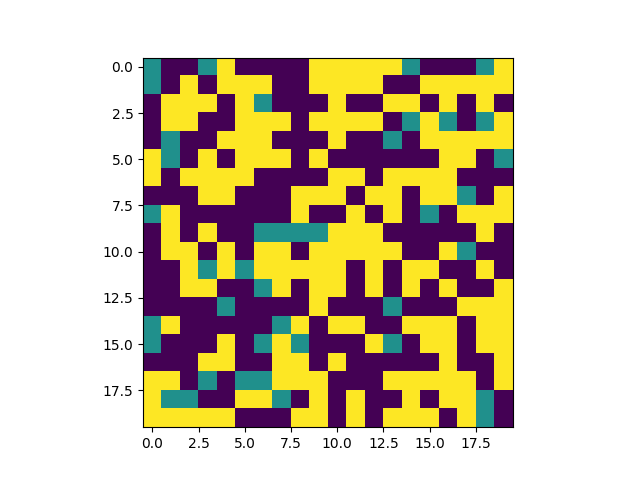
\includegraphics[width=7cm]{../resultats/worlds/Sorted/INS_0.1/sorted_20.png} }}
	\subfloat[Dissatisfaction rate at 0.2]{{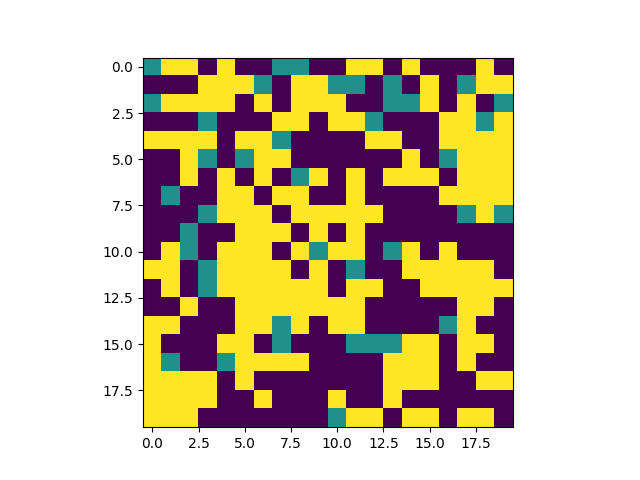
\includegraphics[width=7cm]{../resultats/worlds/Sorted/INS_0.2/sorted_20.png} }}
\end{figure}

\begin{figure}[!h]
	\centering
	\subfloat[Dissatisfaction rate at 0.3]{{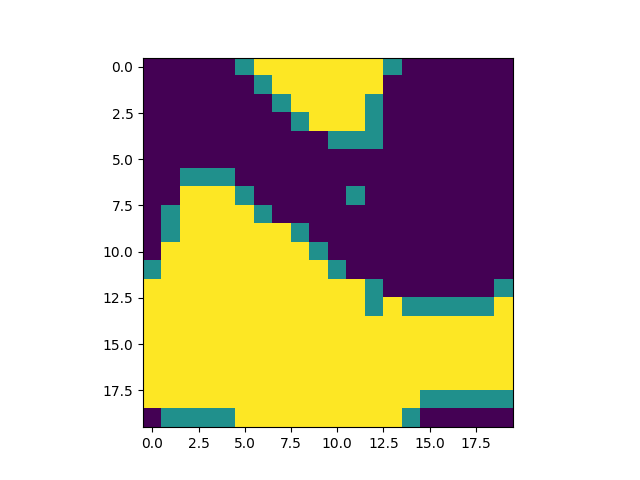
\includegraphics[width=7cm]{../resultats/worlds/Sorted/INS_0.3/sorted_20.png} }}
	\subfloat[Dissatisfaction rate at 0.4]{{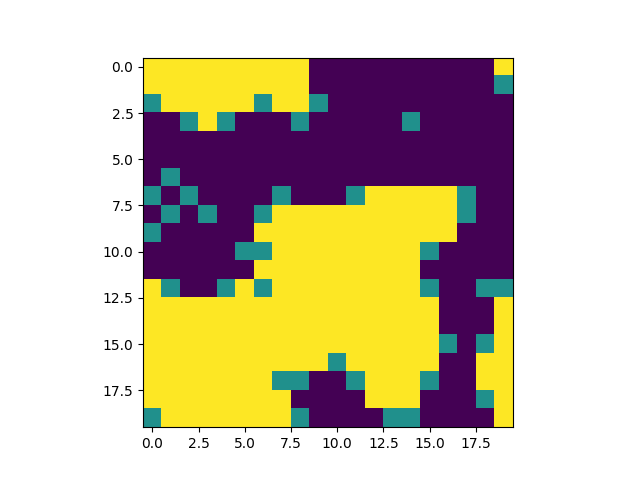
\includegraphics[width=7cm]{../resultats/worlds/Sorted/INS_0.4/sorted_20.png} }}
	\caption{Graphic representation of the organization of populations at the end of the simulations for a given dissatisfaction rate}
\end{figure}


It is clear that whatever the level of dissatisfaction, our agents tend to separate. We observe a limit rate from which this division becomes much more important.
This rate is equal to 1/3 (approximately 0.3). This is a value found by Thomas Schelling which is the threshold from which, whatever the initial conditions,
we will always obtain a segregation of our agents. This law is called the "law of thermodynamics".
\newpage

\begin{figure}[!h]
	\centering
	\subfloat[Population of 200 agents]{{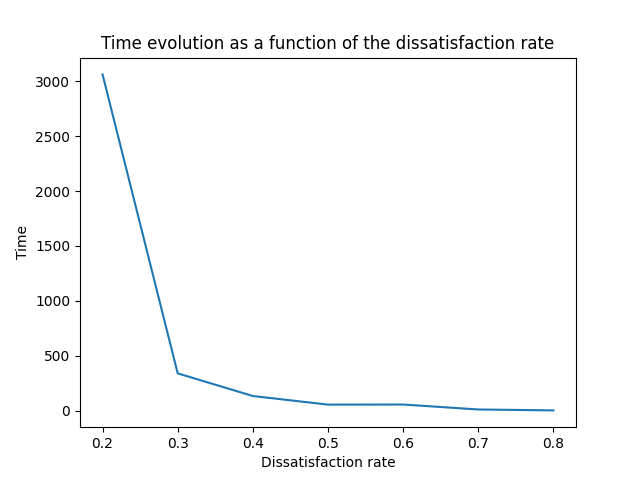
\includegraphics[width=8cm]{../resultats/Curves/INS_evolution/INS_evolution_as_function_of_time_for_POP_200.png} }}
	\subfloat[Population of 205 agents]{{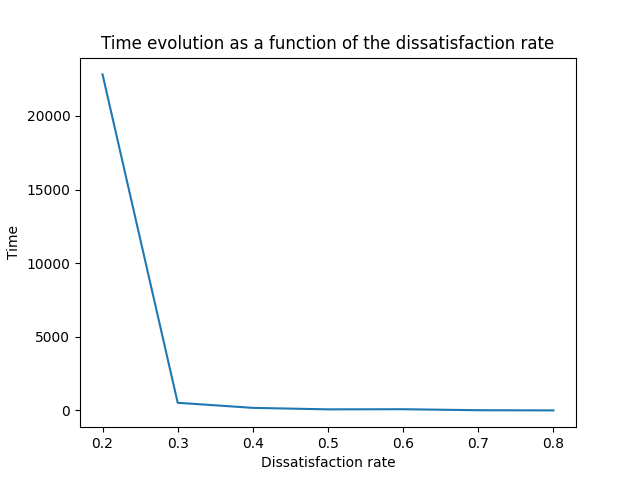
\includegraphics[width=8cm]{../resultats/Curves/INS_evolution/INS_evolution_as_function_of_time_for_POP_205.png} }}
\end{figure}
\begin{figure}[!h]
	\centering
	\subfloat[Population of 210 agents]{{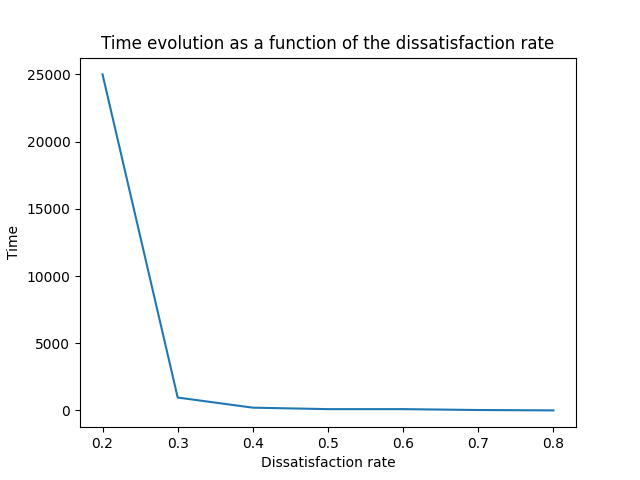
\includegraphics[width=8cm]{../resultats/Curves/INS_evolution/INS_evolution_as_function_of_time_for_POP_210.png} }}
	\caption{Graphical representation of the evolution of the time spent by the agents to reach a stable population separation as a function of the dissatisfaction rate at different population size}
\end{figure}

This law is all the more visible on the curves of the evolution of the time taken by the agents to separate. Indeed, the threshold at 0.3 is clearly represented by
a drastic reduction of the simulations's execution time.

\newpage

\section{Conclusion}

After studying the different cases, we were able to discover that the number of free cells has a big impact on the time of convergence towards a stable situation.
Indeed, the latter is inversely proportional to time. It is therefore possible to deduce that the number of free cells is proportional to the number of occupied cells
and therefore by extension to population density. In addition, we were able to observe that the organization of populations depends on the satisfaction of the agents. Plus an agent
will accept having different neighbors, the shorter the convergence time. And finally, we were able, by our own means, to achieve the same results as Thomas Schelling
and obtain an organization of populations respecting the law of thermodynamics.

\end{document}

